\section{Amplificatore invertente e non-invertente}

\begin{figure}[h!]
\centering
		\begin{minipage}[c]{.4\textwidth}
			\centering

			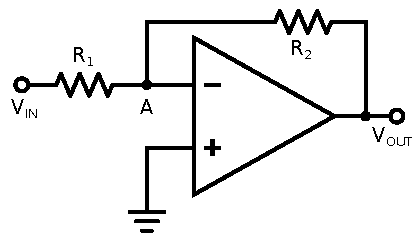
\includegraphics[width=.65\textwidth]{ccinv.pdf}
			\label{fig:ccinv}
			\caption{Amplificatore invertente}

		\end{minipage}%
		\hspace{10mm}%
		\begin{minipage}[c]{.4\textwidth}
			\centering

			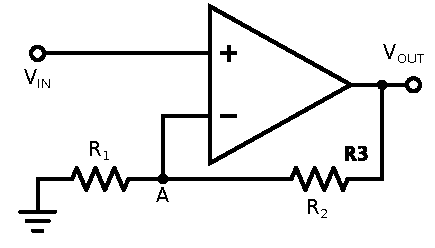
\includegraphics[width=.65\textwidth]{ccninv.pdf}
			\label{fig:ccninv}
			\caption{Amplificatore non invertente}
			
		\end{minipage}
\end{figure}

Il primo circuito da noi analizzato consiste in un amplificatore invertente accoppiato DC.
Lo schema è riportato in Fig.(\ref{fig:ccinv}).
Come vediamo, il nostro amplificatore operazionale è collegato con un circuito di \textbf{feedback} \textbf{negativo} (ovvero viene portato un po' del segnale in output all'ingresso invertente).
Così facendo possiamo avere un controllo sul segnale in uscita che altrimenti sarebbe, per come è costruito l'op-amp, $\pm V$ (avendo un guadagno di $10^6$).

Se consideriamo il nostro amplificatore operazionale ideale, abbiamo che $\Delta V_{12}=0$ (prima condizione di idealità).
Il punto $A$ sarà un ground virtuale.
Possiamo dunque imporre $I_1=\frac{V_{in}-V_A}{R_1}=\frac{V_{in}}{R_1}$.
Inoltre $I_2=\frac{V_A-V_{out}}{R_2}=\frac{-V_{out}}{R_2}$.
Sfruttando la seconda condizione di idealità, $\Delta I_{12}=0$, otteniamo $V_{out}=-\frac{R_2}{R_1} V_{in}$.
Il guadagno del nostro circuito amplificatore sarà dunque:

$$G=-\frac{R_2}{R_1}$$

Esso è negativo in quanto sfasato rispetto al segnale in ingresso di $\pi$.
La richiesta fatta era di ottenere un guadagno di circa -10.
Abbiamo dunque scelto di usare $R_1=(1001.6\pm0.3)\Omega$ e $R_2=(9987.1\pm0.3)\Omega$.
Il circuito è stato alimentato con un segnale in input sinusoidale alla frequenza di 1kHz.
Per valori picco-picco maggiori di $3V$ abbiamo notato l'ormai classico effetto di clapping del segnale, in quanto la tensione in output raggiungeva il valore massimo fornito dalla polarizzazione DC dell'op-amp. 

Ne abbiamo inoltre analizzato l'andamento al variare della frequenza.
Come già accaduto per l'amplificatore alle differenze, abbiamo notato che a frequenze elevato il guadagno diminuiva considerevolmente, con anche uno sfasamento rilevante dei segnali.
In Fig.(\ref{fig:ccninv}) è riportato un grafico del guadagno in funzione della frequenza. 

$$Grafico??$$

$$Se abbiamo i dati$$


Crediamo che il motivo di tale smorzamento del segnale sia la presenza dei transistor e delle capacità nell'amplificatore operazionale.


Successivamente abbiamo montato l'amplificatore non invertende come mostrato in Fig.(\ref{fig:ccninv}). Con gli stessi ragionamenti fatti sopra, possiamo calcolare il guadagno di tale circuito: $V_A=V_{in}=V_{out}\frac{R_1}{R_2+R_1} \Rightarrow V_{out}=(1+\frac{R_2}{R_1})$. Il guadagno, positivo in questo caso, risulta essere: 

$$G=1+\frac{R_2}{R_1}$$

Anche per questo circuito abbiamo analizzato la risposta in frequenza.
Il risultato ottenuto è identico a quello per il circuito precedentemente analizzato e dunque abbiamo deciso di non riportare un grafico.